\section{Introduction}\label{sec:zero-shot-intro}


\begin{figure}
  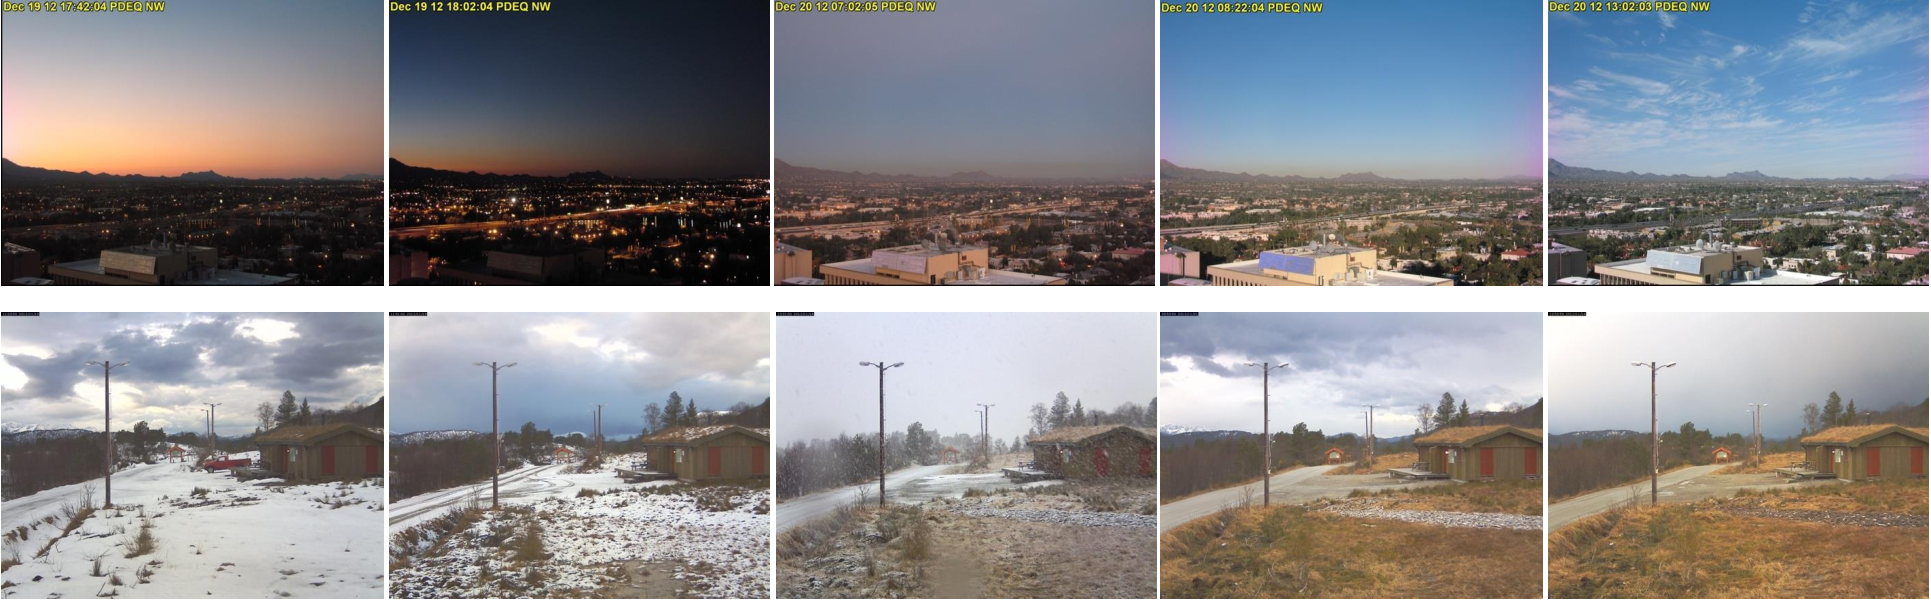
\includegraphics[width=\textwidth]{Chapters/zero-shot-tat-figs/tat-teaser.pdf}
  \caption{Transition of the illumination throughout the day or the weather changes across seasons alter the scene appearance significantly in terms of texture, colour and content. However, some clues, such as the structure, permanent objects, etc. remain unchanged. Transient attribute transfer aims to capture alterations related to such temporal effects. Images from the Transient Attribute Dataset \cite{laffont2014transient}.}
  \label{fig:zero-shot-teaser}
\end{figure}


The visual appearance of outdoor scenes is dynamic, continuously shaped by transient attributes such as lighting, weather conditions, and seasonal changes. These attributes play a crucial role in altering how we perceive the world around us, as they influence the color, texture, and overall atmosphere of a scene. From the gradual transition of daylight to dusk, the formation of fog, to the accumulation of snow on tree branches, these transient factors contribute to the captivating and ever-changing nature of our environment.

In recent years, there has been a growing interest in understanding and manipulating these transient scene attributes within the field of computer vision. The ability to transfer or modify such attributes in images holds significant potential for a wide range of applications, including photography enhancement, virtual reality, and the creation of realistic simulations in video games and films. However, accurately transferring transient attributes between scenes poses a complex challenge, as it requires not only a deep understanding of the scene's inherent structure but also the ability to preserve essential content while adapting to the desired attribute change.

This paper aims to address these challenges by exploring novel methodologies for transient attribute transfer. We build upon recent advancements in generative models and diffusion techniques, leveraging pre-trained models to guide the transfer process in a way that minimizes the risk of overfitting and enhances the generalization capability. Specifically, we focus on developing a zero-shot approach that eliminates the need for extensive additional datasets, instead utilizing the robust priors embedded in foundation models. Our approach is evaluated through a series of qualitative assessments, demonstrating its effectiveness in accurately transferring attributes such as seasonal changes and varying lighting conditions while maintaining the integrity of the scene's core features.

By advancing the understanding and manipulation of transient scene attributes, this research contributes to the broader goal of enhancing the realism and flexibility of visual content generation, paving the way for more immersive and contextually adaptive visual experiences.

In summary, there are two main contributions of this work: 

%Multiple Transformation Blending
\begin{itemize}

    \item \textbf{A novel patch-space image map representation} as a weighted blending of transformation matrices with neural fields.
    
	\item \textbf{A one-shot detail retouching algorithm} that allows transfer of edits to details to new images based on a single before-after image pair.

\end{itemize}
